% !TEX root = ../main.tex

This section will analyze the problem domain of our solution, in order to be able to come up with an optimal implementation. We will analyze the current application, present the actors of the system, define the use cases which have been chosen for the prototype, present the requirements specified for the system, and finally, describe the domain model for the application.

%
%\subsection{GUI Analysis}
%\todo[inline]{maybe we should remove this}
\subsection{Actors}
This section will present the actors of the system. There are four actors of the prototype, the unregistered user, the registered user, location, and Server.

\begin{description}
\item [Unregistered user:] is a user who is not registered in the system i.e. he does not have an account.
\item [Registered user:] also known as ‘user’, is a user, who has an account, and is an active user on the platform.
\item [Location:] is the location of the registered user. This actor is responsible for triggering events when the registered user is near a report.
\item [Server:] is the server which serves the data to the android application, and accesses the database.
\end{description}
These actors will be used in the following section in the use cases, which presents the features of the system.


\subsection{Use Cases}
With the actors from the previous section, we created use cases in order to figure out what services our prototype application should offer.

\begin{enumerate}[label=UC\arabic*]
\item Register user
\item Login
\item Create report
\item Change settings
\item View Report
\item View Leaderboard
\item Validate report
\item Comment on report
\item Display report notification
\item Logout
\end{enumerate}

These use cases can be seen in the use case diagram in \autoref{fig:uc_diag}. The use case diagram shows the relation between actors and use cases, and shows what actors have access to which use cases.

\begin{figure}[hbt]
\centering
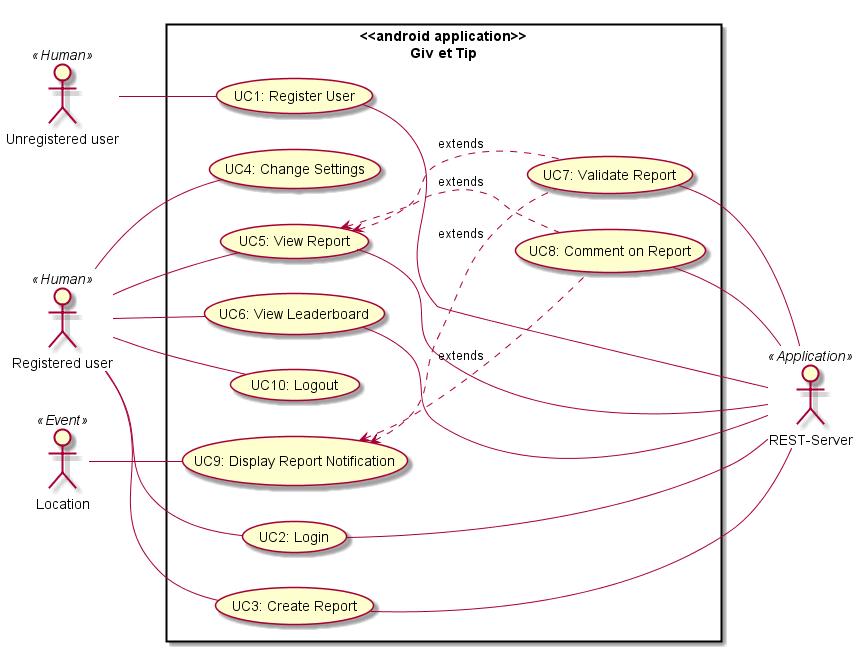
\includegraphics[width=\textwidth]{images/use_case_diagram}
\caption{Use case diagram for the system} \label{fig:uc_diag}
\end{figure}

\subsubsection{Use Case Descriptions}~\\
\noindent This section will describe the use case UC9 into greater detail. For descriptions of all use cases look in \appref{app:ucd}.

\autoref{tab:uc9} shows the description of UC9. It shows the main flow with its alternative flows, which ends the flow. The reason for the alternative flows to end the use case, is that this is supposed to happen in the background, and the user should not be interrupted, unless there actually is something to notify him about.
% UC9
\begin{table}[htb]
%\todo[inline]{check for the positioning of this one (UC9 desc)}
\caption{Use case description for UC9.}\label{tab:uc9}
\begin{tabularx}{\textwidth}{|l|X|}
\hline
Name              & Display Report Notification \\ \hline 
Id                & UC9 \\ \hline
Description       & Allows the application to send notifications to the user, if he is within his set distance threshold of a report. \\ \hline
Primary Actors    & Location \\ \hline
Secondary Actors  & NA \\ \hline
Preconditions     & The user has location services enabled. \\ \hline
Main Flow         &
{\footnotesize \begin{enumerate}
\item The distance from the user’s current location is within the set threshold
\item The application checks if the user has already contributed to this report.
\begin{enumerate}
\item Alternative flow: Alternative Flow: User already contributed to report:
\end{enumerate}
\item The application checks if the user has been shown this report before
\begin{enumerate}
\item Alternative Flow: Report already shown.
\end{enumerate}
\item The application gets the latest information about the report.
\begin{enumerate}
\item Alternative Flow: No connection to server.
\end{enumerate}
\item The user is asked to validate the report.
\item end.
\end{enumerate}} \\ \hline
Postconditions    & A notification is shown to the user, and he can respond to ut with UC7 or UC8. \\ \hline
Alternative Flows & 
User already contributed to report:
{\footnotesize \begin{enumerate}
\item end.
\end{enumerate}}
Report already shown:
{\footnotesize \begin{enumerate}
\item end.
\end{enumerate}}
No connection to Server:
{\footnotesize \begin{enumerate}
\item end.
\end{enumerate}}
\\ \hline
\end{tabularx}
\end{table}

This section has introduced the use cases, which has been worked with within this project. These use cases will be used in the following section to lay basis for some of the requirements to the system.

\subsection{Requirements}
This section defines the requirements set up for the prototype system. These requirements has been based upon the use cases from the previous sections, and based on the development knowledge within the team.

The requirements has been divided into the Functional and Nonfunctional requirements.

\subsubsection{Functional Requirements}~\\
The functional requirements are the requirements which defines the functionality of the system. The functional requirements can be seen in the list below.

\begin{enumerate}[label=F\arabic*]
\item Unregistered users should be able to register as users.
\item The user should be able to login to their account.
\item The user should be able to logout of their account.
\item The user should be able to create a report.
\item The user should be able to change the location of the report.
\item The user should be able to change the distance threshold to reports, for notifications.
\item The user should be able to view reports inside the application.
\item The user should be able to view the user points leaderboard.
\item The user should be able to validate a report bu voting up or down for it.
\item The user should be able to comment on reports.
\item The system should notify the user, whenever he is within the distance threshold of a report, and ask for a validation.
\end{enumerate}

\subsubsection{Nonfunctional Requirements}~\\
The nonfunctional requirements has been divided into what parts of the system they belong to, e.g. the requirements for the server is in the server category, and the requirements for the mobile application is in the mobile application category.
The categories and requirements can be seen in the lists below.

\newpage
\paragraph{Server}
\begin{enumerate}[label=NS\arabic*]
\item The Server should be RESTful, in order to serve both the application and a web client.
\item The Server should be able to run on Debian linux.
\item The server should be developed in java.
\item The server should have a connection to a MySQL database.
\end{enumerate}

\paragraph{Mobile application}
\begin{enumerate}[label=NA\arabic*]
\item The application should be developed with minimum SDK 23.
\item The application should use as little powers as possible.
\item The application should contain a user friendly UI.
\item The application should show the reports on a map.
\item The application should check the distance to nearby reports in the background.
\item The application should hash all passwords, using the SHA-256 algorithm.
\end{enumerate}


The key requirements, which is necessary in order to solve the problems, which this project focuses on, are the following:

\textbf{NA5}, without this the application will not be able to ask the users to verify reports, \textbf{F10} is directly dependent on this requirement.

\textbf{F8} and \textbf{F9}, without these functional requirements ensures that there will be features for verifying the reports.


\subsection{Domain Model}
The domain model is a conceptual model of our platform. It identifies objects or entities in the real world which will be a part of the system.

\begin{figure}[hbt]
\centering
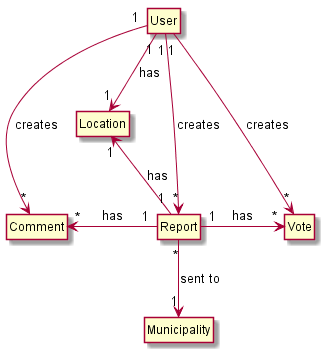
\includegraphics[width=.375\textwidth]{images/domain_diagram}
\caption{The Domain model for the Giv et Tip prototype} \label{fig:dom_diag}
\end{figure}


\autoref{fig:dom_diag} shows a simple domain model for our prototype, we can see the user can create reports, comments and votes, and has a location. We can see the report has comments, votes and a location, and that the report is sent to the municipality, which is represented by the Server actor.

\vspace{3em}
\hrule
In this analysis section the actors of the system have been identified, the use cases, which has been used throughout the development phase of the prototype system, have been discovered, the requirements to the system has been established, and the domain model have been presented.